\documentclass[a4paper, 12pt]{article}
\usepackage[slovene]{babel}
\usepackage[utf8]{inputenc}
\usepackage[T1]{fontenc}
\usepackage{lmodern}
\usepackage{graphicx}
\usepackage{amssymb}
\usepackage{amsmath}
\usepackage{mathtools}
\setlength{\parindent}{0px}
\setlength{\parskip}{10px}
\usepackage{enumitem}
%\usepackage{blindtext}
\usepackage{lipsum}
\usepackage{scrextend}
\usepackage{array}
\usepackage{tikz}
\usepackage[margin=1in]{geometry}
\usetikzlibrary{shapes,arrows}
\usepackage{listings}
\usepackage{color}
\usepackage{multirow}
\usepackage[
colorlinks=true,
linkcolor=black,
anchorcolor=black,
citecolor=black,
filecolor=black,
menucolor=black,
runcolor=black,
urlcolor=black
]{hyperref}

\title{Zapiski iz pouka Osnove programiranja II Programiranje Mikrokontrolerjev}
\author{Matej Blagšič}

\begin{document}

%---------------------------------------------------za diagrame
\tikzstyle{decision} = [diamond, draw, fill=blue!20, 
text width=4.5em, text badly centered, node distance=3cm, inner sep=0pt]
\tikzstyle{block} = [rectangle, draw, fill=blue!20, 
text width=5em, text centered, rounded corners, minimum height=4em]
\tikzstyle{line} = [draw, -latex']
\tikzstyle{cloud} = [draw, ellipse,fill=red!20, node distance=3cm,
minimum height=2em]
\tikzstyle{nothing} = [draw, node distance =3cm]

%-------------------------------------za programiranje text barvanje
\definecolor{dkgreen}{rgb}{0,0.6,0}
\definecolor{gray}{rgb}{0.5,0.5,0.5}
\definecolor{mauve}{rgb}{0.58,0,0.82}
\definecolor{lgray}{RGB}{250,250,250}
\lstset{
	frame=l,%single
	language=C,
	aboveskip=3mm,
	belowskip=3mm,
	showstringspaces=false,
	columns=flexible,
	basicstyle={\small\ttfamily},
	numbers=none,
	numberstyle=\tiny\color{gray},
	keywordstyle=\color{blue},
	commentstyle=\color{dkgreen},
	stringstyle=\color{mauve},
	breaklines=true,
	breakatwhitespace=true,
	tabsize=4,
	backgroundcolor=\color{lgray},
	moredelim=**[is][\color{dkgreen}]{@}{@}
}
%---------------------------------------//
\newcommand{\harpoon}{\overset{\rightharpoonup}}


\maketitle
\thispagestyle{empty}
\pagebreak
\setcounter{page}{1}

\tableofcontents
\pagebreak



\section{Osnovno}

Pri temu predmetu bomo obravnavali jezik C. Za uporabo lahko preneseš okolje Codeblocks z MinGW inštalacijo ali posebej MinGW compiler in poljubno okolje(Jetbrains).\

Pomembno je, da imaš predznanje iz prejšnjega polletja pri Javascriptu, saj so tipi spremenljivk, sintaksa in drugo zelo podobno, tako da v detajle o stvarih, ki so enake ne bom šel.

Vsak dokument začnemo z \framebox{\lstinline|@#include <stdio.h>@|\par} za standardne vhodne in izhodne ukaze.

Vsa koda se izvaja znotraj main funkcije:

\begin{lstlisting}
int main(){
    printf("Hello!\n");
    return 0;
}
\end{lstlisting}

\textbf{Prav tako je pomembno uporabiti PODPIČJE za vsakim ukazom/vrstico!!!}

Če začnemo na začetku, opazimo \texttt{\#include} ukaz. Ta se izvrši, preden se karkoli drugega. V temu primeru lahko vnesemo knjižnice. Te nam olajšajo programiranje s tem, da nam en ukaz izvede več ukazov, ki bi jih morali tipkati na roke. To datoteko/knjižnico navedemo lahko z "datoteka" navednicam. Če pa damo v <datoteka>, potem pa išče datoteke v sistemskih mapah okolja. Te datoteke so vrste \textbf{header} s končnico \textbf{.h}. V našem primeru je knjižnica za pisat in brat podatke - vhodne in izhodne podatke.\\
To je podobno kot v javascriptu:  \lstinline|<script src="datoteka">|\ 
\section{Podatki}
Poglejmo si zgled:
\begin{lstlisting}
int main(){
	int a;
	float b; //spremenljivka

	printf("Vprisi prvo vrednost");
	scanf("%d", &a);
	printf("Vpisi drugo vrednos");
	scanf("%f", &b);
	printf("%d + %f = %f\n", a, b, a+b);
	return 0;
}
\end{lstlisting}

C je občutljiv na tip podatkov. Pravimo tudi, da je C statično tipiziran jezik. To pomeni, da moramo vrsto podatka navesti. 
To pomeni, da se moramo sami odločiti, kakšen tip podatka bo nosila spremenljivka.

Vemo, da v Javascriptu nismo rabili napisati tipa spremenljivke, le \texttt{var}, torej je Javascript dinamično tipiziran jezik.

\subsection{Branje podatkov}
Da nam program prebere podatek, uporabimo funkcijo:

\begin{center}
	\framebox{\lstinline|scanf("formatno\_dolocilo", \&spremenljivka);|}
\end{center}

Vidimo, da moramo najprej deklarirati tip podatka, ki ga pričakuje operator Scanf. Potem pa določimo naslovni operator \& in nato za njim spremenljivko, ki naj sprejme podatek.

\subsection{Pisanje podatkov}
Za pisanje podatkov uporabimo funkcijo:
\begin{center}
	\framebox{\lstinline|printf("formatni\_niz", izrazi)|}
\end{center}
Pomembne so tudi ubežne sekvence. To so \verb|\r \n \t|, ki povejo, kaj se zgodi, ko se text izpiše. \verb|\n| naredi novo vrstico(new line) po besedilu, \verb|\t| je tabulator...

Tako v našem primeru, se a izpiše tam, kjer je njegov \verb|%d| in b, kjer je \verb|%f| ter vsota $a + b$ tam, kjer je \verb|%f| (glej izsek programske kode).

\subsection{Spremenljivke:}
\begin{table}[!htbp]
	\centering
	\begin{tabular}[b]{|p{3cm}|p{3cm}|p{3cm}|p{4.5cm}|}
		\hline \textcolor{blue}{TIP} & \textcolor{blue}{DOLŽINA(bitov)} & \textcolor{blue}{FORMATNO DOLOČILO} & \textcolor{blue}{OBMOČJE} \\ \hline\hline
		\textcolor{violet}{char} & 8 & \verb|%d %c| & $-128$ do $127$ \\
		\multirow{2}{*}{\textcolor{violet}{short, int}} & 16 & \multirow{2}{*}{\texttt{\%d}} & $-65536$ do $+65535$ \\
		& 32 && $-32768$ do $+23767$ \\
%		32  & \%d &$-65536$ do $+65535$ \ $-32768$ do $+23767$\\
		\textcolor{violet}{long} & vsaj 32 & \verb|%ld| & $-2.1\times10^9$ do $+2.1\times10^9$\\
		\textcolor{violet}{float} & običajno 32 & \verb|%f| & $-2.1\times10^9$ do $+2.1\times10^9$\\
		\textcolor{violet}{double} & običajno 64 & \verb|%lf| & $-9.2\times10^{18}$ do $+9.2\times10^{18}$ \\
		\textcolor{violet}{void} & 0 & & \\ \hline
	\end{tabular}
	\caption{Tipi spremenljivk v c-ju}
\end{table}
%
V C-ju Boolov tip ne obstaja, tako da primerjalni operatorji delujejo enako, le da vračajo 0 za false in 1 za vse, kar je različno od nič. \textbf{Ne obstaja TRUE ali FALSE}.\

Spoznali bomo tudi, da je pri celoštevilskem tipu pomembna omejitev območja, pri realnem tipu pa natačnost!

Velikokrat bomo srečali izraz \lstinline|unsigned|. ta nam območje podatkovnega tipa prestavi od 0 do $2\times$ maksimum. Če je char od -128 dp 127, potem je unsigned char od 0 do 255;

\subsection{Celoštevilski tip (n bitov)}
Obstaja nepredznačen, ki je od 0 do $2^{32}$

\subsection{Realni tip (IEEE floating point)}
\begin{table}[!htbp]
	\centering
	\begin{tabular}{|l|l|l|}
		\hline \textcolor{blue}{p} & \textcolor{blue}{eksp. (e)} & \textcolor{blue}{mantisa (m)} \\ \hline
		1 bit & 8 bitov & 23 bitov \\ \hline
	\end{tabular}
\end{table}

Ta ima enojno natančnost (single precision) ali \emph{\texttt{float}} in so števila zapisana z 32 bitno velikostjo. Tako so v desetiškem sistemu števila natančna do 7,22 signifikantnih mest, sepravi 7 mest je natančnih, od 8. števila naprej pa je že vprašljivo. Torej, signifikantno pomeni pomembno, tisto, kar je natančno.\

Če hočemo večjo natančnost, uporabimo \emph{\texttt{double}} oz. dvojna natačnost (double precision). Ima kapaciteto 64 bitov, torej v desetiškem do 15,95 mest natančno. Po 15. mestu je že vprašljivo natančno.


\subsection{Modifikatorji formatna določila}
\verb|%d| vemo, da stoji za cela števila. Če vrinemo neko število ``N'' $\to$ \texttt{"\%Nd"}, potem povemo, na koliko mest se izpiše število, deluje na desno poravnavo.\\
Če vrinemo ničlo $\to$ \texttt{"\%0Nd"}, potem zapolne prazna mesta z ničlam.\\
Če vrinemo "N.Mf" $\to$ \texttt{"\%N.Mf"}, potem izpiše $N$ mest število z $M$ mesti za decimalno piko.

\begin{lstlisting}
int x = 15;
float y = 3.141592;

printf("%5d",x); --> Izpise _ _ _1 5
printf("%.2f",y); --> Izpise 3.14
printf("%05d",x); --> Izpise 00015
\end{lstlisting} 

\subsection{Znaki}
Imamo več standardov znakov. Najbolj osnoven in razširjen je \texttt{ASCII} (American standard code for information Interchange). Ta zapis je 8-biten. Lahko najdemo tabelco, ki nam pokaže kodo za vsak znak.

\begin{figure}[h!]
	\centering
	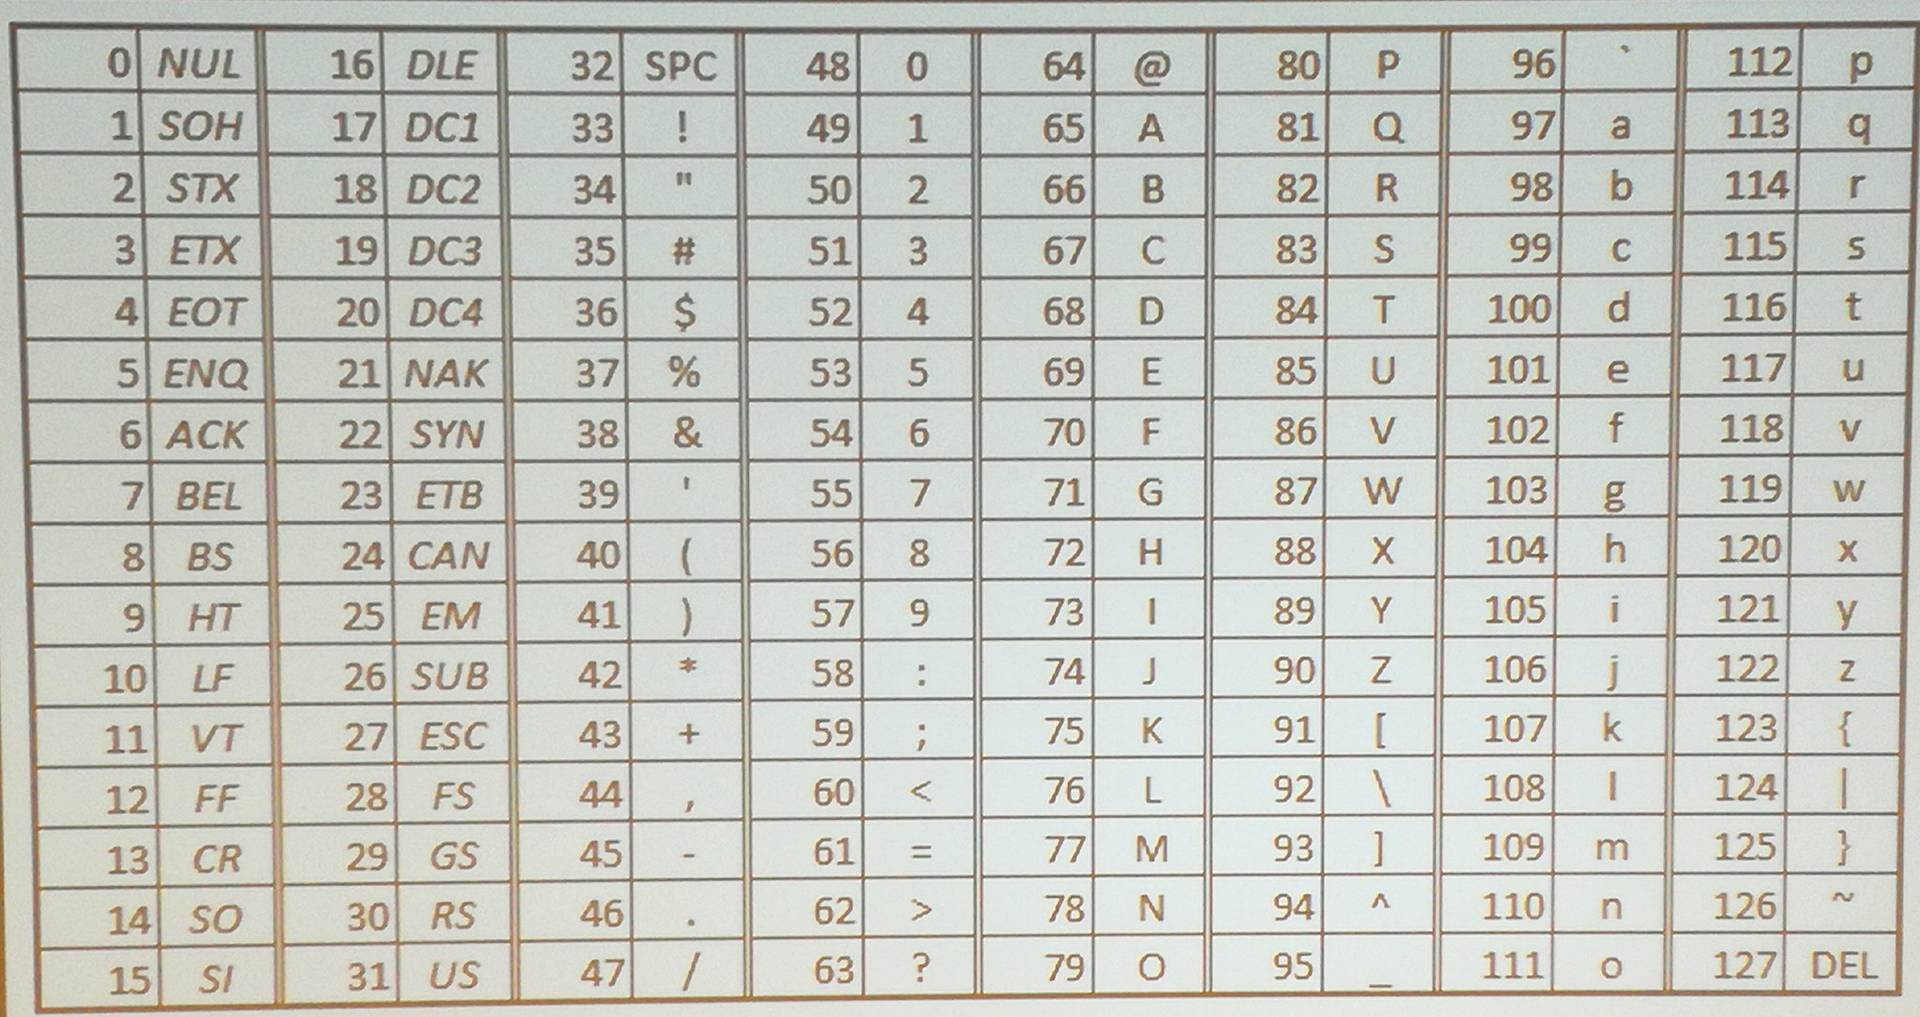
\includegraphics[width=0.7\linewidth]{images/ascii.jpg}
	\caption{ASCII tabela}
	\label{fig:ascii-tabela }
\end{figure}

V C-ju je pomembno, da damo en znak v enojne navednice. S tem pomeni, da program zaznava ASCII kodo. Torej, če izpišemo \lstinline|printf("%d", '0');|, nam program izpiše 48. Pri znakih uporabimo torej spremenljivko \lstinline|char|.

\subsection{Psevdonaključna števila}
Ena metoda za pridobivanje naključnih števil je metoda srednjih kvadratov.
Pri tem kvadriramo dvomestna števila. Pri tem je statistično gledano naključnost zelo podobna realni naključnosti, kot da bi metali kocke.

\subsection{Statične in dinamične spremenljivke}
\textbf{Glej priloženo kodo spodaj!}

V temu programu imamo funkcijo tipa void, ki kot vemo ne vrne nič, pred funkcijo main. prav tako imamo definirano spremenljivko ga, ki je zunaj kode. Ta je zato globalna in je uporabna v vseh funkcijah. Te globalne spremenljivke so \textbf{STATIČNE}. To pomeni da so te spremenljivke vedno na voljo in hranijo vrednost ves čas, kajti prostor za njih je že rezerviran v začetku.

Za kontrast, vse lokalne spremenljivke so \textbf{DINAMIČNE}, razen če so definirane kot statične z ukazom \lstinline|static| pred definicijo spremenljivke(glej kodo, vrstica 6). Če poženemo kodo vidimo, kako deluje ukaz static. Ker smo spremenljivko \textcolor{purple}{sa} definirali le enkrat in ji dodali vrednost 12, potem se ne definira ponovno vsakič, ko pridemo v to funkcijo \textcolor{green}{foo()} še enkrat. Zato se vrednost te spremenljivke povečuje. Za kontrast, spremenljivka \textcolor{purple}{a} se ne povečuje, saj se vsakič, ko pridemo v funkcijo \textcolor{green}{foo()} ponovno definira.

Prav tako velja, da statične neinicializirane spremenljivke dobijo vrednost 0. To ne velja za dinamične, tako da če ne zapišemo začetne vrednosti spremenljivke \textcolor{purple}{a}, potem vidimo, da program meče za vrednosti \textcolor{purple}{a} kar nekaj.

\begin{lstlisting}
#include <stdio.h>
int ga; //globalna spremenljivka

void foo(){
	int a = 12;	//lokalni spremenljivki
	static int sa = 12; //spremenljivka je staticna
	a++;
	sa++;
	ga++;
	printf("%d, %d, %d\n", ga, a, sa);
}
int main(){
	for(int i=0; i < 5; i++){
		foo();
	}
	return 0;
}	
\end{lstlisting}
\subsection{Zbirka(array)}
Pomnilnik je razdeljen na pomnilniške celice v velikosti 8 bitov na celico. Ko naslavljamo celico, je vedno naslednja celica za 1 večja od prejšne po vrstni številki. \

\begin{center}
	\framebox{\lstinline|tipElementa imeZbirke[dim] = \{element1, element2, element3, ...\}|}
\end{center}

V temu primeru, je ,,dim'' dimenzija zbirke. Naslavljamo jih lahko enako, kot v javascriptu, to je, da napišemo ime zbirke in "stevilo, ki predstavlja mesto želenega elementa. Ne moremo izpisati celotne zbirke naenkrat, temveč le po en element naenkrat. Pomembno je tudi, da ena zbirka določenega tipa lahko vsebuje elemente le tega tipa, torej vsi enaki. Ne moremo mešati različnih tipov, kot v javascriptu.

Poglejmo si zanimiv primer:

\begin{lstlisting}
#include <stdio.h>

int a[] = {2, 4};
int b[] = {1, 3};

int main(){

	a[2] = 42;
	b[-1] = 42;

	printf("%d, %d", a[1], b[0]);

	return 0;
}
\end{lstlisting}

V tem primeru, imamo globalna arraya $a$ in $b$. Imata dva elementa, torej je njuna velikost 2. Nato pa v main funkciji elementu 2 v arrayu $a$ in elementu -1 v arrayu $b$ priredimo vrednost 42. In potem, ko izpišemo drugi člen arraya $a$ in prvi člen arraya $b$, se nam izpišeta točno te dve števili. Zelo je čudno, saj ne mormo iti v negativno mesto arraya, drugo mesto arraya pa ne obstaja, saj pri obeh gre le 0 in 1. mesto.

"Zal na predavanjih "se nismo (niste) obdelali kazalcev. Zakaj se to zgodi pojasnijo kazalci. Spremenljivki $a$ in $b$ sta v resnici kazalca na za"cetek seznamov, ki sta jima prirejena. $a$ torej ka"ze na prvi element v seznamu in ko kli"cemo \lstinline|a[0]| v resnici zahtevamo element, ki se nahaja na mestu, na katerega ka"ze a, plus 0. Torej element na za"cetku seznama. Ko kli"cemo \lstinline|a[1]| tako zahtevamo element, ki se nahaja na mestu na katerega ka"ze $a$ plus 1. Torej naslednji element. Ve"c o kazalcih in seznamih si lahko prebere"s  \href{https://github.com/DzinVision/c-uvod}{\texttt{na tej povezavi}}.

Seznama  \lstinline|a| in \lstinline|b| pa imata v tem primeru "se eno lastnost -- deklarirana sta en za drugim ter vsebujeta zelo malo elemntov. Zaradi tega se seznam \lstinline|b| na RAM-u nahaja takoj za seznamom \lstinline|a|. Ko pokli"cemo \lstinline|a[2]| gremo v resnici na prvi element v seznamu \texttt{b}, ko pokli"cemo \lstinline|b[-1]|, pa gremo v resnici na zadnji element seznama \texttt{a}. Ko kasneje izpi"semo zadnji element seznama \texttt{a} in prvi element seznama \texttt{b}, se izpi"seti to"cno te "stevili. 

Ker v obeh primerih nastavimo "stevilo v seznamu na 42, lahko dobimo la"zen ob"cutek, da se v vrstici \lstinline|a[2]| "stevec obrne in gremo nazaj na prvo mesto v seznamu \texttt{a}, v vrstici \lstinline|b[-1]|, pa da gre "stevec od zadaj in pi"semo na zadnje mesto v seznamu \texttt{b}. Da se to v resnici ne zgodi, lahko preverimo na zelo preprost na"cin -- vsakemu seznamu nastavimo druga"cno "stevilo. Poglejmo si naslednjo kodo.

\begin{lstlisting}
#include <stdio.h>

int a[] = {2, 4};
int b[] = {1, 3};

int main(){
	a[2] = 42;
	b[-1] = 69;

	printf("%d, %d", a[1], b[0]);

	return 0;
}
\end{lstlisting}

Ta program bo sedaj izpisal \texttt{69 42}, torej smo res z \lstinline|b[-1]| nastavili zadnji element v \texttt{a}, z \lstinline|a[2]|, pa smo nastavili prvi element v \texttt{b}.
%
\subsection{Znakovni niz(string)}
V C-ju ne ovstaja string kot samostojen tip. Ampak vemo, če poznamo zbirke in char, da je string nič drugega kot zbirka char elementov. Zato lahko definiramo string kot v prvem ali drugem okvirčku. Prvi je namreč bolj kot zbirka, a težje za vnašanje:
\begin{center}
	\framebox{\lstinline|char niz[] = {'a','b','c','d' ..... 'n'}|}
	\framebox{\lstinline|char niz[] = "abcd....n"|}
\end{center}

Lahko definiramo tudi drugače, kot je zapisano v drugem okvirčku.

Poglejmo primer. Imamo program, ki nam izpiše string kot posamezne elemente zbirke txt v for zanki. For zanka je napisana malo drugače. Namesto primerjave v srednjem delu, imamo primerjavo $i$-tega člena zbirke txt in če je ta različna od nič oz. če obstaja, zato lahko tam napišemo ali: \texttt{txt[i] != 0} ali pa \texttt{txt[i]}, potem jo izpiše. Tako se pomika po zbirki navzgor. Na koncu vsake zbirke, je "nevidna" ničla in ko jo najde, jo več ne izpiše in se for zanka konča. Jaz sem uporabil drugo metodo.

\begin{lstlisting}
#include <stdio.h>

int main(){
	char txt[] = "Tole izpisi";
	for (int i = 0; txt[i]; i++){
		printf("%c", txt[i]);
	}
	return 0;
}
\end{lstlisting}

Ker se string rabi pogosto, obstaja formatno določilo \textcolor{purple}{\%s}. Tako lahko napišemo program kot kaže koda. Pomni, da ko izpišeš, uporabi le ime char array-a brez oglatih oklepajev.

\begin{lstlisting}
#include <stdio.h>

int main(){
	char txt[] = "Tole izpisi";
	printf("%s", txt); // <-- tu txt, ne txt[] ter formatno dolocilo %s
	return 0;
}
\end{lstlisting}

\section{Operatorji}
Pri C-ju so enaki operatorji, kot v JS, le da z nekimi izjemami: Operator === in !=== ne obstajata.\\
Prav tako operator za deljenje ne zapišemo kot ``/'' ne deluje enako. Problem prihaja iz tipa spremenljivk. Če obsoječo spremenljivko $x$, ki je tipa \underline{int}, deljimo ali spreminjamo tako, da bi postala ta spremenljivka kateregakoli drugega tipa, kot prvotni \underline{int}, potem vrne program 0. Primer:
\begin{lstlisting}
int maint(){	
	x = 7;
	x = x / 8 * 8
	
	printf("%d", x);
	return 0;
}
\end{lstlisting}
Če pa spremenimo prvo 8 z 8.0, potem bo program jo vzel za realno število in deljil in nato nazaj množil z 8, tako se te pokrajšata in program vrne 7.

\section{Funkcije}
Funkcije deklariramo tako:

\begin{center}
	\framebox{\underline{tip\_funkcije} \lstinline| imeFunkcije()\{/*telo funkcije*/	return 0;\}|}
\end{center}

Opazimo, da funkcijo deklariramo kot float oz. funkcijo, ki vrne realno število. V resnici lahko funkcije definiramo kot karkoli hočemo, glede na to, kaj naj bi vrnila.

Prav tako vidimo, da glavna zanka, v kateri se koda izvaja, je \texttt{main}. v tej kodi se izvajajo vsi programi in funkcije. Tako se koda, ki je napisana tu notri, se prevede in spremeni v izvršilno kodo(executable).

Primer funkcije je iz poglavja Psevdonaključna števila. Tam smo spoznali definiranje funkcije:
\framebox{\lstinline|int dogodek(float verjetnost);|} Vidimo, da moramo za razliko od JS definirati vrsto spremenljivke, ki gre v vhodne podatke, tj. verjetnost. Poleg tega, ker se konča z podpičjem, imenujemo ta del prototip. Nič ne naredi. Nato definiramo šele funkcijo.

\begin{lstlisting}
#include <stdio.h>
#include <stdlib.h>
#include <time.h>

int dogodek(float verjetnost);
int dogodek(float verjetnost){
	if((float)rand() / RAND_MAX <= verjetnost){}
		return 1;
	}
}
int main(){

	int x, stevec = 0;
	srand(time(NULL));
	for(x=0; x < 100000;x++){
		stevec += dogodek(0.5);
	}
	printf("%d", stevec);

	return 0;
}
\end{lstlisting}

V funkciji je pomembno, da pretvorimo rand() v float tip spremenljivke, ker drugače gre za celoštevilsko deljenje, kar potem pomeni le 0 ali 1. Problem je, da nam potem vsakič vrne enako vrednost okoli 50 000, ker je ta random le psevdonaključna. Zato srednjo verednost definiramo z ukazom \texttt{srand}(oz seme) in vanj vnesemo čas, ki pa nikoli ni enak. Zato tako vsakič generira zares naključno število.

Naredimo primer na bolezni. Izračunajmo, koliko \% ljudi, ki so bolani zares, zanje test pokaže, da so res bolani.

Testiramo 100 000 ljudi in vemo, da bolezen ubije 0.5\% ljudi. Prav tako vemo, da test pokaže z natančnostjo 99\%, da je oseba bolana. 1\%, da je oseba zdrava. Ampak ali je res, da je 1\% zdravih ali napačno diagnosticirano.

\begin{lstlisting}
int main(){

    unsigned long i;
	float pBolan = 0.005; //verjetnost da ubije
	float pPozitBolan = 0.99; //resnicno bolan verjetnost
	float pPozitZdrav = 0.01;//verjetnost da pokaze da je bolan, ceprav je zdrav
	unsigned long pozit = 0;
	unsigned long pozitBolan = 0;
	
	srand(time(NULL));
	for(i = 0; i<100000;i++){
		if(dogodek(pBolan)){//vemo da je bolan
			if(dogodek(pPozitBolan)){//testiramo kako dobro izmerimo,ce je bolan
				pozitBolan++;//dodamo ga med bolane in pozitivno testirane
				pozit++;
			}
		}
		else{//testiramo zdravega
			if(dogodek(pPozitZdrav)){//tu se znajde zdrav in pozitivno testiran
				pozit++;
			}
		}
	}
	printf("%f", (float)pozitBolan/pozit);// rezultat je bolni/testirane pozitivno
}
\end{lstlisting}

\section{Strukture}

V C-ju, za razliko od C++ in JS ni objektov. Zato imamo strukture, ki so nekako podobna zadeva. Definiramo z :
\begin{lstlisting}
struct ime{
	tip1 ime1;
	tip2 ime2;
	...
};
\end{lstlisting}
Struct s spremenljivko ime je nov podatkovni tip. In ko definiramo komponente tega novega podatkovnega tipa, definiramo novo spremenljivko kot:
\framebox{\lstinline|struct ime sprem;|}

Če hočemo klicati spremenljivko, definiramo kot \lstinline|sprem.ime1;| Glej kodo spodaj za referenco:

\begin{lstlisting}
#include <stdio.h>

struct vektor {
	float x, y;		
};

int main() {
	struct vektor v1, v2;

	v1.x = 1.4;	
	v1.y = -0.7;

	v2 = v1;  // ustvari se cista kopija, ne samo povezava do spremenljivke, kot v JS
	v2.x = 13;
	printf("%d\n", v1.x == v2.x);  // testiramo, da vidimo, ali je enakost, %d, ker nam vraca 1 ali 0(boolean)
	
	return 0;
}
\end{lstlisting}

Primer uporabe  je sledeča koda. Napišemo program, ki nam izračuna vektorski produkt dveh vektorjev. Vektorski produkt dveh vektorjev vemo, da je nov vektor, ki je pravokoten na prvotna dva $\vec{a}$ in $\vec{b}$. Vektorski produkt lahko rešimo z determinanto $3 \times 3$ matrike vektorjev. Po definiciji sledi:
\begin{equation*}
\vec{a} \times \vec{b} = 
\begin{vmatrix}
\vec{i} & \vec{j} & \vec{k} \\
a_x & a_y & a_z\\ 
b_x & b_y &b_z \notag
\end{vmatrix} = 
\begin{bmatrix}
a_y\cdot b_z - a_z\cdot b_y \\
a_z\cdot b_x - a_x\cdot b_z \\
a_x\cdot b_y - a_y\cdot b_x
\end{bmatrix} = 
\begin{bmatrix}
x \\ 
y \\ 
z
\end{bmatrix}
\end{equation*}

\end{document}